\section{Fitness Function}
The fitness function is the essential part of the GA that assess the solutions. The target solutions lie on the extreme value of the fitness and it does not matter if it is maximum or minimum. There are no rule for its range of values and only simple recommendations for its creation. The target value of average maintained illuminance and the target value of uniformity are watched in the algorithm. The output design is the most effective and the cheapest after the target values are reached with minimum count of luminaires. Therefore the minimalization of the luminaires count is also expected.

First attempt to create suitable fitness function was based on the idea, that the least count of luminaries was got for the exact target value of illuminace. The fitness function consists of sum of two parts $g_1$, $g_2$ defined as follows:

\begin{equation}
\label{eq:fitV1}
f\left(\overline{E}_{m}, U_0\right) = g_1\left(\overline{E}_{m}\right) + g_2\left(U_0\right)
\end{equation}

\begin{equation}
\label{eq:fitV1G1}
	g_1\left(\overline{E}_{m}\right)=
	\begin{cases} 
		e^{\frac{\overline{E}_{m}-\overline{E}_{mT}}{\overline{E}_{m}}} & \left( 0, \overline{E}_{mT}\right\rangle\\
		e^{\frac{\overline{E}_{mT}-\overline{E}_{m}}{\overline{E}_{m}}} & \left( \overline{E}_{mT}, \infty\right)
	\end{cases}
\end{equation}

\begin{equation}
\label{eq:fitV1G2}
	g_2\left(U_0\right)=
	\begin{cases} 
		\frac{U_0}{2\cdot U_{0T}} & \left\langle 0, U_{0T}\right\rangle\\
		1-\frac{e^{\frac{U_{0T}-U_0}{U_{0T}}}}{2} & \left( U_{0T}, \infty\right)
	\end{cases}
\end{equation}

\noindent where:
\begin{description}
	\item[$\overline{E}_{m}$] is a calculated maintained average value of illuminance,
	\item[$\overline{E}_{mT}$] is a target maintained average value of illuminance,
	\item[$U_0$] is a calculated lighting uniformity,
	\item[$U_{0T}$] is a target lighting uniformity.
\end{description}

The exponential function were used in both parts. Each part could reach maximum of $1$. The Function~\ref{eq:fitV1G1} respected the requirements for target illuminance. The maximum was reached exactly for target value of illuminance. As it can be seen from Figure~\ref{fig:fitV1G1G2}, according to the definition the higher values of illuminance were preferred because there was a slower change of the function for this part of interval. The limits at both bounds of definition interval reached zeros:

\begin{equation}
\label{eq:g1lim0}
\lim_{\overline{E}_{m}\to 0+} g_1\left(\overline{E}_{m}\right) = 0
\end{equation}
\begin{equation}
\label{eq:g1limInf}
\lim_{\overline{E}_{m}\to \infty} g_1\left(\overline{E}_{m}\right) = e^{-1}
\end{equation}

The Function~\ref{eq:fitV1G1} respected the requirements for uniformity and it was linear until it reached the target value. Then the exponential function created the saturation effect.

According to designed fitness function, the algorithm was supposed to reach the target value of illuminance with the highest possible uniformity. However only the restriction of getting exact value of the illuminance was not sufficient to get least count of luminaires. The demand of maximum uniformity favored solutions with little bit more luminaires. Although this fact could be fixed by adding weight multiplier to one of the part given by Equation~\ref{eq:fitV1G1} or \ref{eq:fitV1G2}, the function did not seem to be further suitable for the algorithm and optimization. Especially it could hardly include any preferences from designer and the calculations of exponential functions were time consuming.

\begin{figure}[htb]
  \centering
  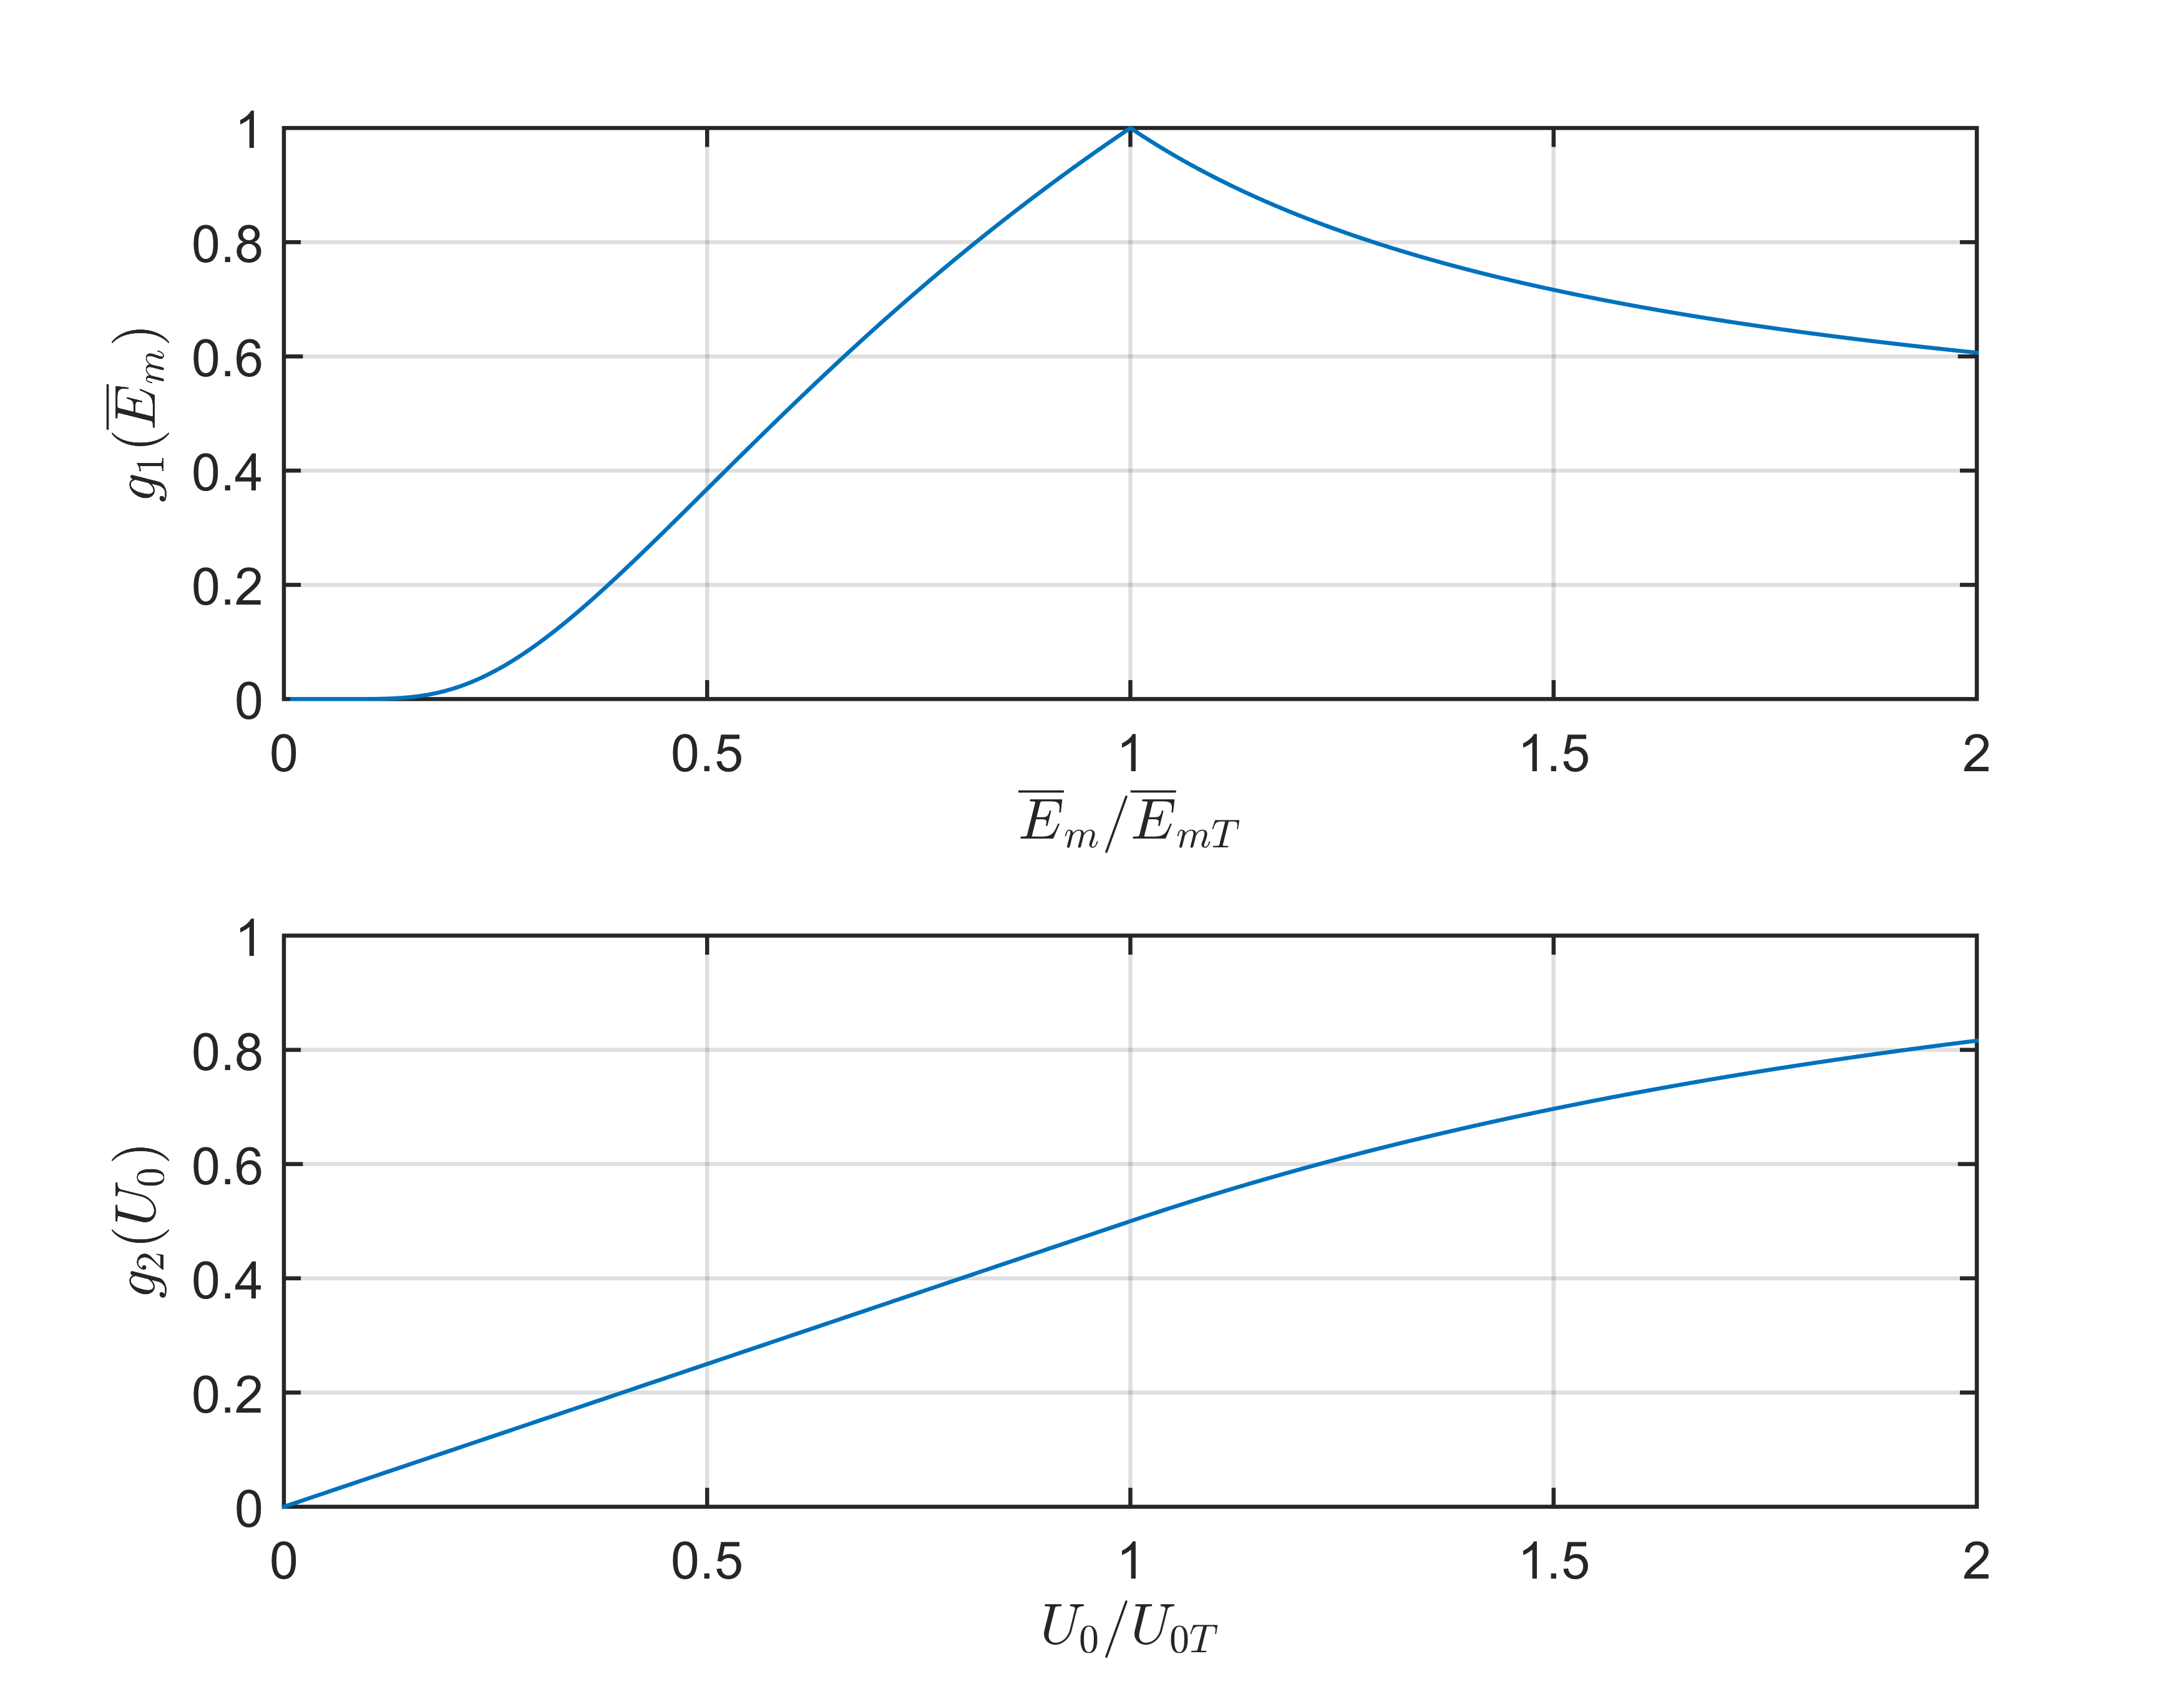
\includegraphics[width=\columnwidth]{obrG1G2}
  \caption{Graphs of parts $g_1\left(\overline{E}_{m}\right)$ and $g_2\left(U_0\right)$ from the fitness function}
  \label{fig:fitV1G1G2}
\end{figure}

The fitness function bellow is currently used in the algorithm. Solutions that does not reach basic requirements of target illuminance or uniformity are valued by length of the chromosome $L$:

\begin{equation}
\label{eq:fitV2EUA}
	f\left(C,\overline{E}_{m}, U_0\right)= L
\end{equation}

\noindent Otherwise the fitness is evaluated by:

\begin{equation}
\label{eq:fitV2EUB}
\begin{split}
f\left(C, \overline{E}_{m}, U_0\right)&=C +\\
& + \left( 1 - \alpha\right)\cdot\frac{\overline{E}_{mT}}{\overline{E}_{m}+\epsilon} + \\
& + \alpha\cdot\frac{U_{0T}}{U_0 + \epsilon}
\end{split}
\end{equation}

\noindent where:
\begin{description}
	\item[$C$] is count of luminaires,
	\item[$\overline{E}_{m}$] is a calculated maintained average value of illuminance,
	\item[$\overline{E}_{mT}$] is a target maintained average value of illuminance,
	\item[$U_0$] is a calculated lighting uniformity,
	\item[$U_{0T}$] is a target lighting uniformity,
	\item[$\alpha$] is number between 0 and 1,
	\item[$\epsilon$] is a very small number, that prevents the division by 0.
\end{description}

The $\alpha$ represents the designer intention to prefer one of the parameter to another. Target ratio between relative values of the parameters can be get from partial derivation of the fitness function:

\begin{equation}
\label{eq:fitV2ratio}
\frac{\overline{E}_{m}}{\overline{E}_{mT}}\cdot\frac{U_{0T}}{U_0}=\sqrt{\frac{1-\alpha}{\alpha}}
\end{equation}

\noindent There is no preference if $\alpha$ is equal to $0.5$.

This fitness function is supposed to be minimized. The Equation \ref{eq:fitV2EUB} can be at the point close to the target values of illuminance and uniformity separated into integer part, that is only given by count of luminaires $h_1\left(C\right)= C$ and fraction part that is given by:

\begin{equation}
\label{eq:fitV2frac}
	h_2\left(\overline{E}_{m}, U_0\right)= \left( 1 - \alpha\right)\cdot\frac{\overline{E}_{mT}}{\overline{E}_{m}+\epsilon} + \alpha\cdot\frac{U_{0T}}{U_0 + \epsilon}
\end{equation}

The main impact of the integer part $h_1\left(C\right)$ occurs at the beginning of the optimization. Only solutions that fulfill the standard requirements can have smaller value of fitness than the length of chromosome. For other solutions is the most effective way to minimize the Equation~\ref{eq:fitV2EUB} decreasing the count of luminaires. Changes in the part $h_2\left(\overline{E}_{m}, U_0\right)$ are less significant, because for high counts of luminaires, the denominator of the Equation~\ref{eq:fitV2frac} is much higher than the numerator. Therefore the resulting fraction is very small.

After getting optimal count of luminaires, the part $h_2\left(\overline{E}_{m}, U_0\right)$ takes values less than but quite close to one. The effective way of minimize the Equation~\ref{eq:fitV2EUB} is to get the highest possible illuminance and uniformity for given count of luminaires then.

The defined fitness function was used for several runs of GA and it always worked well. However there is known problem in the definition of Equation~\ref{eq:fitV2EUA}. Consider the case, that any of initial solutions does not fulfil the standard requirements. Then all of them have the same  fitness value equal to length of the chromosome $L$. It is very probable, that after selection, crossovers and mutations at least one solution fulfilling the standard requirements appears. But there can also be rare  cases, that the algorithm never optimizes the count of luminaires, because the fitness function is independent on all parameters for solutions here. The presence of the problem is more probable for very small population sizes, small count of generations, small probability of mutations or inappropriately designed selection method.

There can be added some parameter dependency in Equation~\ref{eq:fitV2EUA}. However it was quite useless for further described settings of GA and chosen selection method. It would be extremely rare if any of the solutions fulfilling standard requirements did not appear after couple of generations.
